
\subsection{Red de una empresa}
Este experimento sobre una red Wi-Fi en una empresa con alrededor de 15 empleados. En esta red se suelen conectar varios dispositivos móviles y también notebooks.

\subsubsection{Fuente S}

Utilizando las herramientas presentadas en el ejercicio 1 sobre esta red se obtuvieron los siguientes resultados
\begin{itemize}
 \item $12039$ paquetes unicasts
 \item $6561$ paquetes broadcasts
 \item $18600$ paquetes en total
\end{itemize}

 La \emph{entropía} para esta fuente se calculó en  $0.936493026389$. El siguiente gráfico muestra este comportamiento. \par
 %\textbf{METER EL GRAFIQUITO DE LA ENTROPIA UNICAST Y BROADCAST}

%\blindtext

\begin{figure}[H]
   \centering
       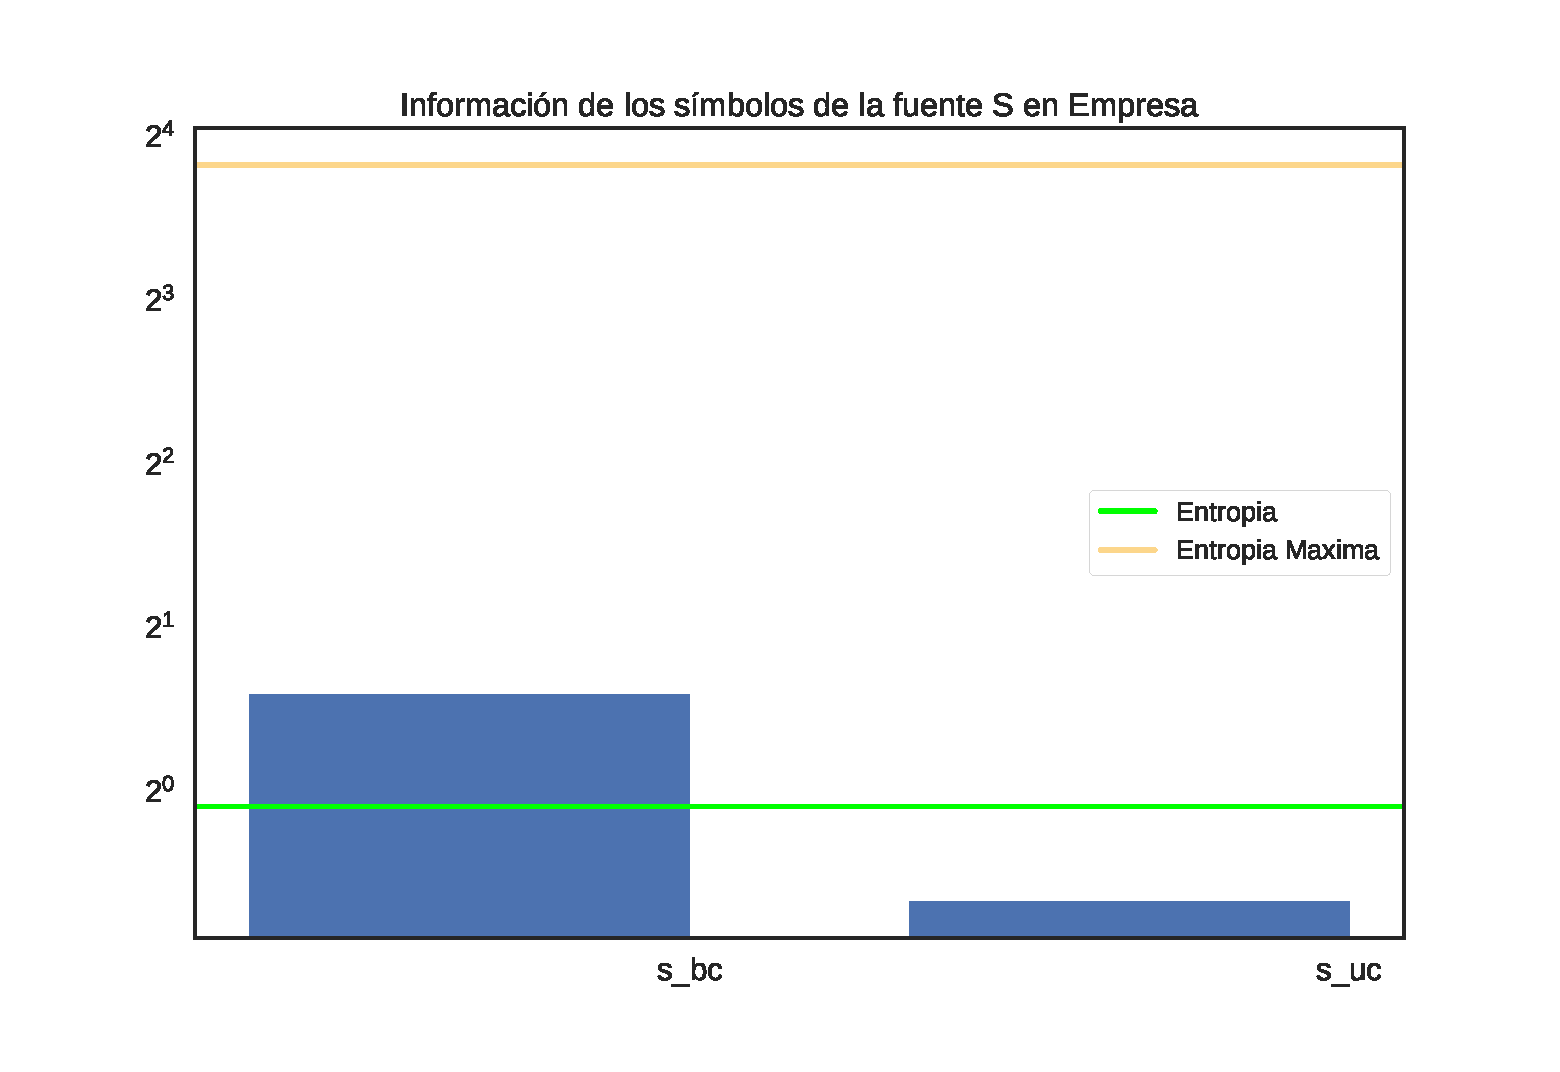
\includegraphics[page=1,width=.70\textwidth]{../img/barras-Empresa} &
 \caption{Entropía de la red}
 \label{fig:Test}
\end{figure}

%\blindtext




 Como la medición se realiza sobre una red inalámbrica a la cual se encuentran conectados varios dispositivos, es razonable que exista una mayor presencia de paquetes \emph{unicast}. Esto es porque dichos dispositivos, generalmente, envían paquetes a un destino IP particular con la finalidad de conectarse a algún servidor externo. \par


\subsubsection{Grafo de conectividad de la red}


\begin{figure}[H]
   \centering
       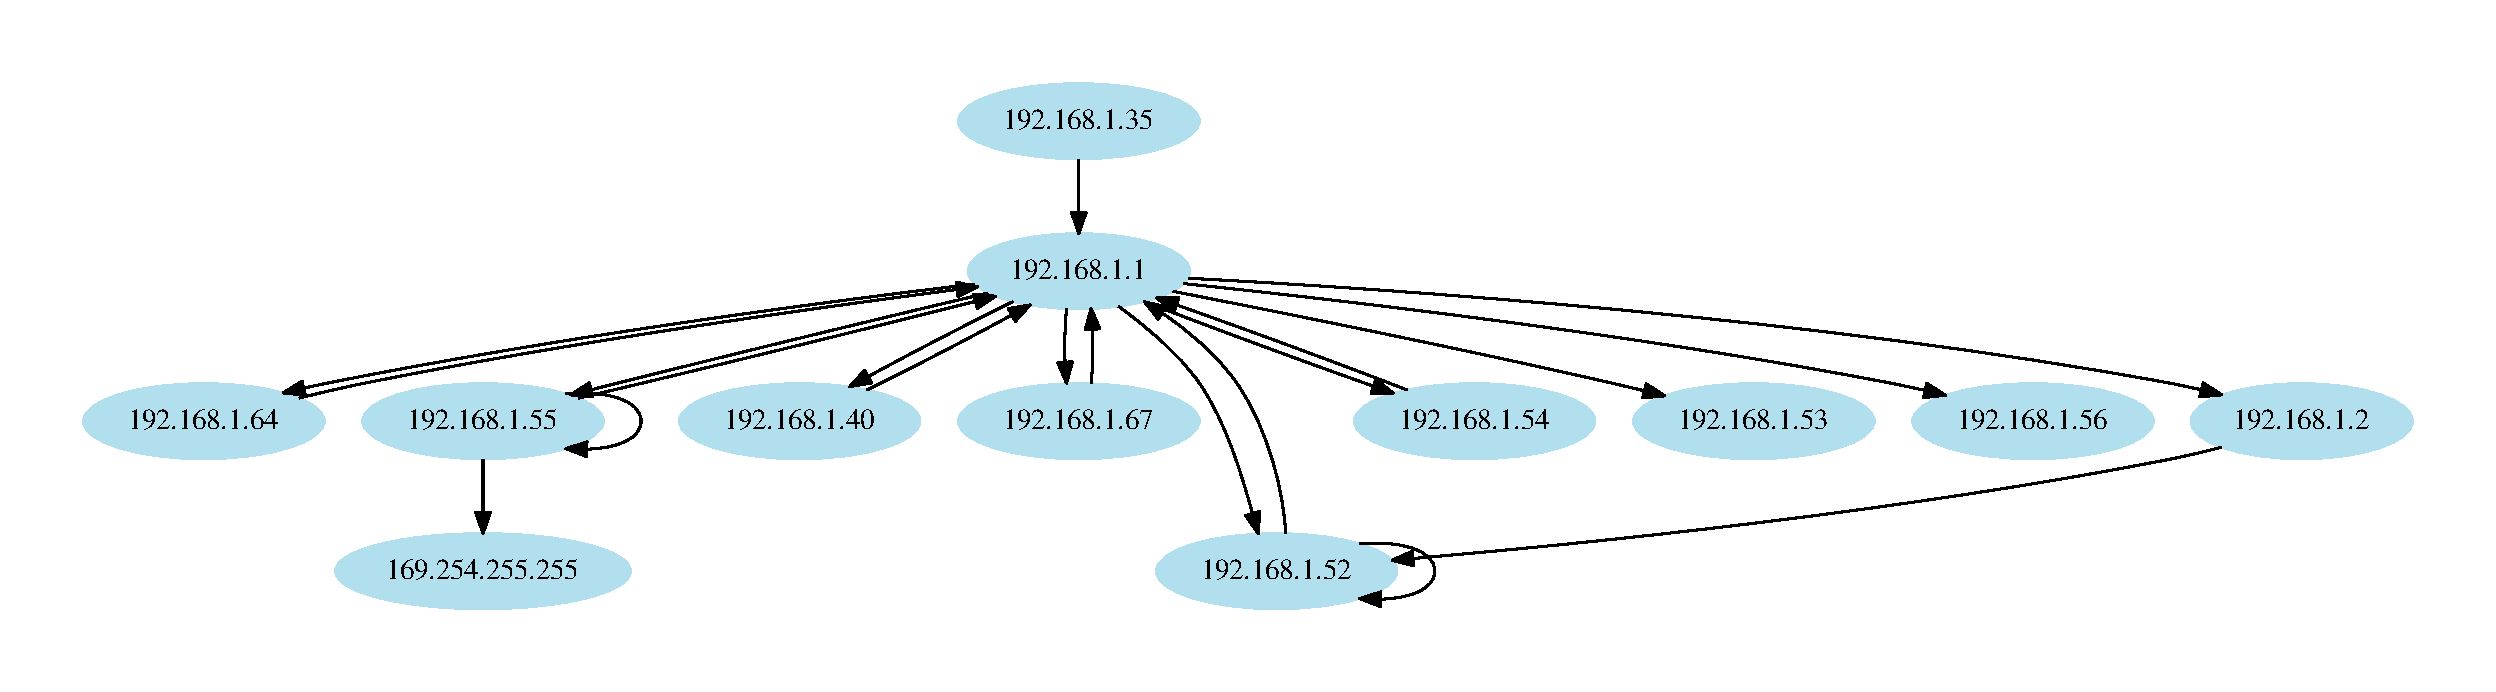
\includegraphics[page=1,height=8cm ,width=1.08\textwidth]{../img/red-Empresa} &
 \caption{Grafo de conectividad}
 \label{fig:Test}
\end{figure}

% \textbf{GRAFICO!!}

 En la figura anterior se puede observar que el nodo 192.168.1.1 se comporta como un nodo raíz al cual se conectan varios dispositivos, este comportamiento es esperado debido a que se trata de una red Wi-Fi en el cual el nodo 192.168.1.1 podría ser el Router. \\

A su vez, se puede observar que las direcciones asignadas son de la forma 192.168.1.0 con una máscara $/25$ ya que ninguno de los \emph{hosts} tiene asignado direcciones superiores a $126$. \\

También se puede observar un pedido de asignación de IP por parte del host 192.168.1.55 hacia el servidor DHCP (169.254.255.255).\\

Por último podemos observar paquetes en las cuales la dirección de destino coincide con la dirección del emisor, esto se debe a que son \emph{gratuitous ARP packets} los cuales suponemos son utilizados para anunciar a la red de la presencia de un nuevo dispositivo o para actualizar las tablas de ARP luego de que una MAC address cambia de IP.


 \subsubsection{Información y nodos distinguidos}
 Para esta sección reutilizamos la herramienta presentada en el ejercicio 2 con el objetivo de analizar la presencia de nodos distinguidos de la fuente. \\

 Como se puede observar en la figura \ref{fig:distinguidos-empresa}, el dispositivo 192.168.1.1 se comporta como único nodo distinguido de nuestra red y su dirección se corresponde con las asignadas generalmente por los routers, por este motivo no es precipitado suponer que podría tratarse del \emph{default gateway} de esta red.

\begin{figure}[H]
   \centering
       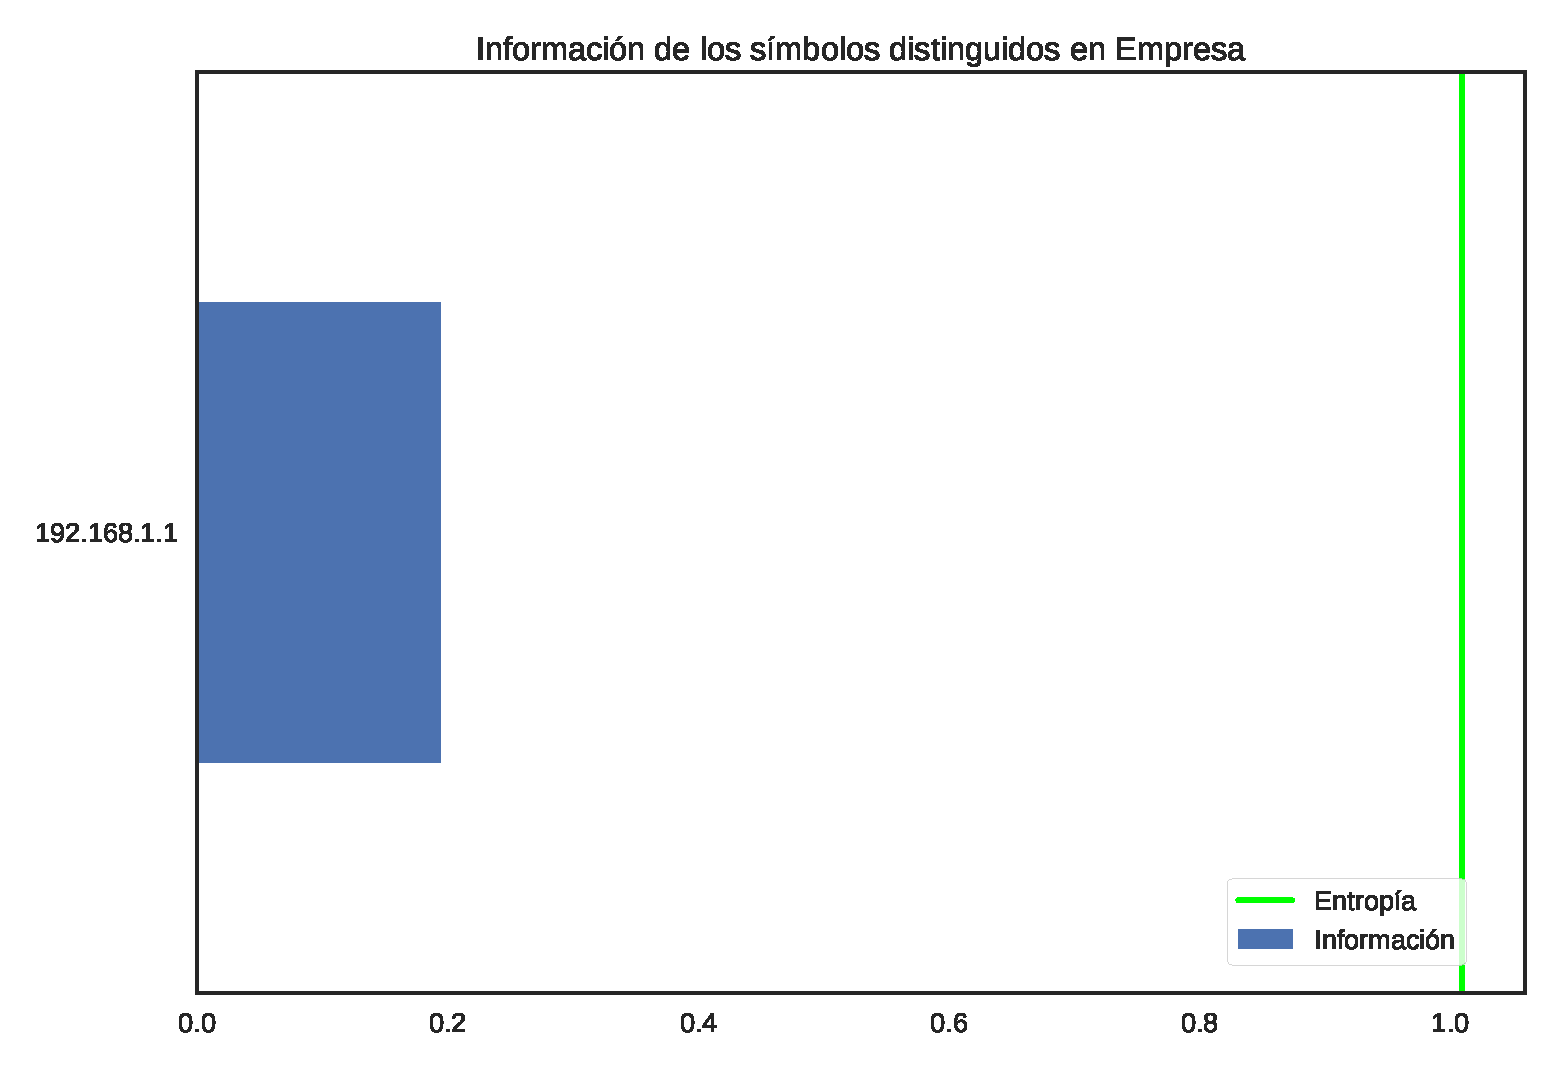
\includegraphics[page=1, height=6.8cm ,width=\textwidth]{../img/distinguidos-Empresa} &
 \caption{Nodos distinguidos}
 \label{fig:distinguidos-empresa}
\end{figure}


% \textbf{GRAFQUITO DEL NODO DISTINGUIDO}
